\documentclass[a4paper, 12pt]{article}
\usepackage[utf8]{inputenc}
\usepackage[T1]{fontenc}
\usepackage[spanish]{babel}
\usepackage{amsmath}
\usepackage{amsfonts}
\usepackage{amssymb}
\usepackage{graphicx}
\usepackage{hyperref}
\usepackage{siunitx}
\usepackage{caption}
\usepackage{subcaption}
\usepackage{xcolor}
\hypersetup{colorlinks=true, linkcolor=blue!50!black, urlcolor=gray!70!black}

\title{Informe de construcción de Divisor de Potencia de Wilkinson}
\author{Leila Scerbo, Simón Aulet}
\date{Julio 2025}
\begin{document}
\maketitle

\begin{abstract}
Este informe detalla el proceso de diseño, simulación y construcción de un divisor de potencia de Wilkinson balanceado para operar a \SI{1}{\giga\hertz}. Se presentan los fundamentos teóricos, las simulaciones electromagnéticas, el proceso de fabricación mediante router CNC y las mediciones finales realizadas con un analizador de redes vectoriales.
\end{abstract}

\section*{Diseñamos un divisor de potencia de Wilkinson balanceado}

\section*{Principio de funcionamiento}
Se trata de dividir una señal de entrada en dos señales cada una con una fracción de la potencia usando dos transformadores de $\frac{1}{4}$ de onda para adaptar la impedancia de entrada al circuito. La relación entre la potencia de entrada $P_1$ y las potencias de salida de cada puerto $P_2$ y $P_3$ viene dada por la razón de división de potencia $k = \sqrt{P_2/P_3}$ resultando en:
\begin{equation}
Z_{01} = Z_0 \sqrt{1 + k^2}
\end{equation}
\begin{equation}
Z_{02} = Z_0\sqrt{1 + \frac{1}{k^2}}
\end{equation}

En nuestro caso usamos $P_2 = P_3 = \frac{P_1}{2}$ resultando en:
\begin{equation}
Z_{01} = Z_{02} = Z_0 \cdot \sqrt{2}
\end{equation}

Entonces cada salida debe reflejar un 50\% de la potencia de entrada quedando:
\begin{equation}
P_2 = P_3 = P_1 / 2 \Rightarrow 10\log\left(\frac{P_2}{P_1}\right) = -3\text{dB}
\end{equation}

\section*{Proceso de diseño}
\subsection*{Materiales y equipamiento}

\subsubsection*{PCB}
\begin{minipage}{0.66\linewidth}
  El proyecto se va a imprimir sobre una placa para radiofrecuencia \cite{RT-DUROID}con las siguientes características:
  \begin{tabular}{|l|l|l|}
  \hline
  Parámetro & Valor & \\ \hline
  Constante dieléctrica & $2.00 \pm 0.04$ & \\ \hline
  Espesor del dieléctrico & $0.05$ inch & \\ \hline
  Espesor del cobre ($t$) & $35 \mu m$ & \\ \hline
  \end{tabular}
\end{minipage}
\begin{minipage}{0.32\linewidth}
  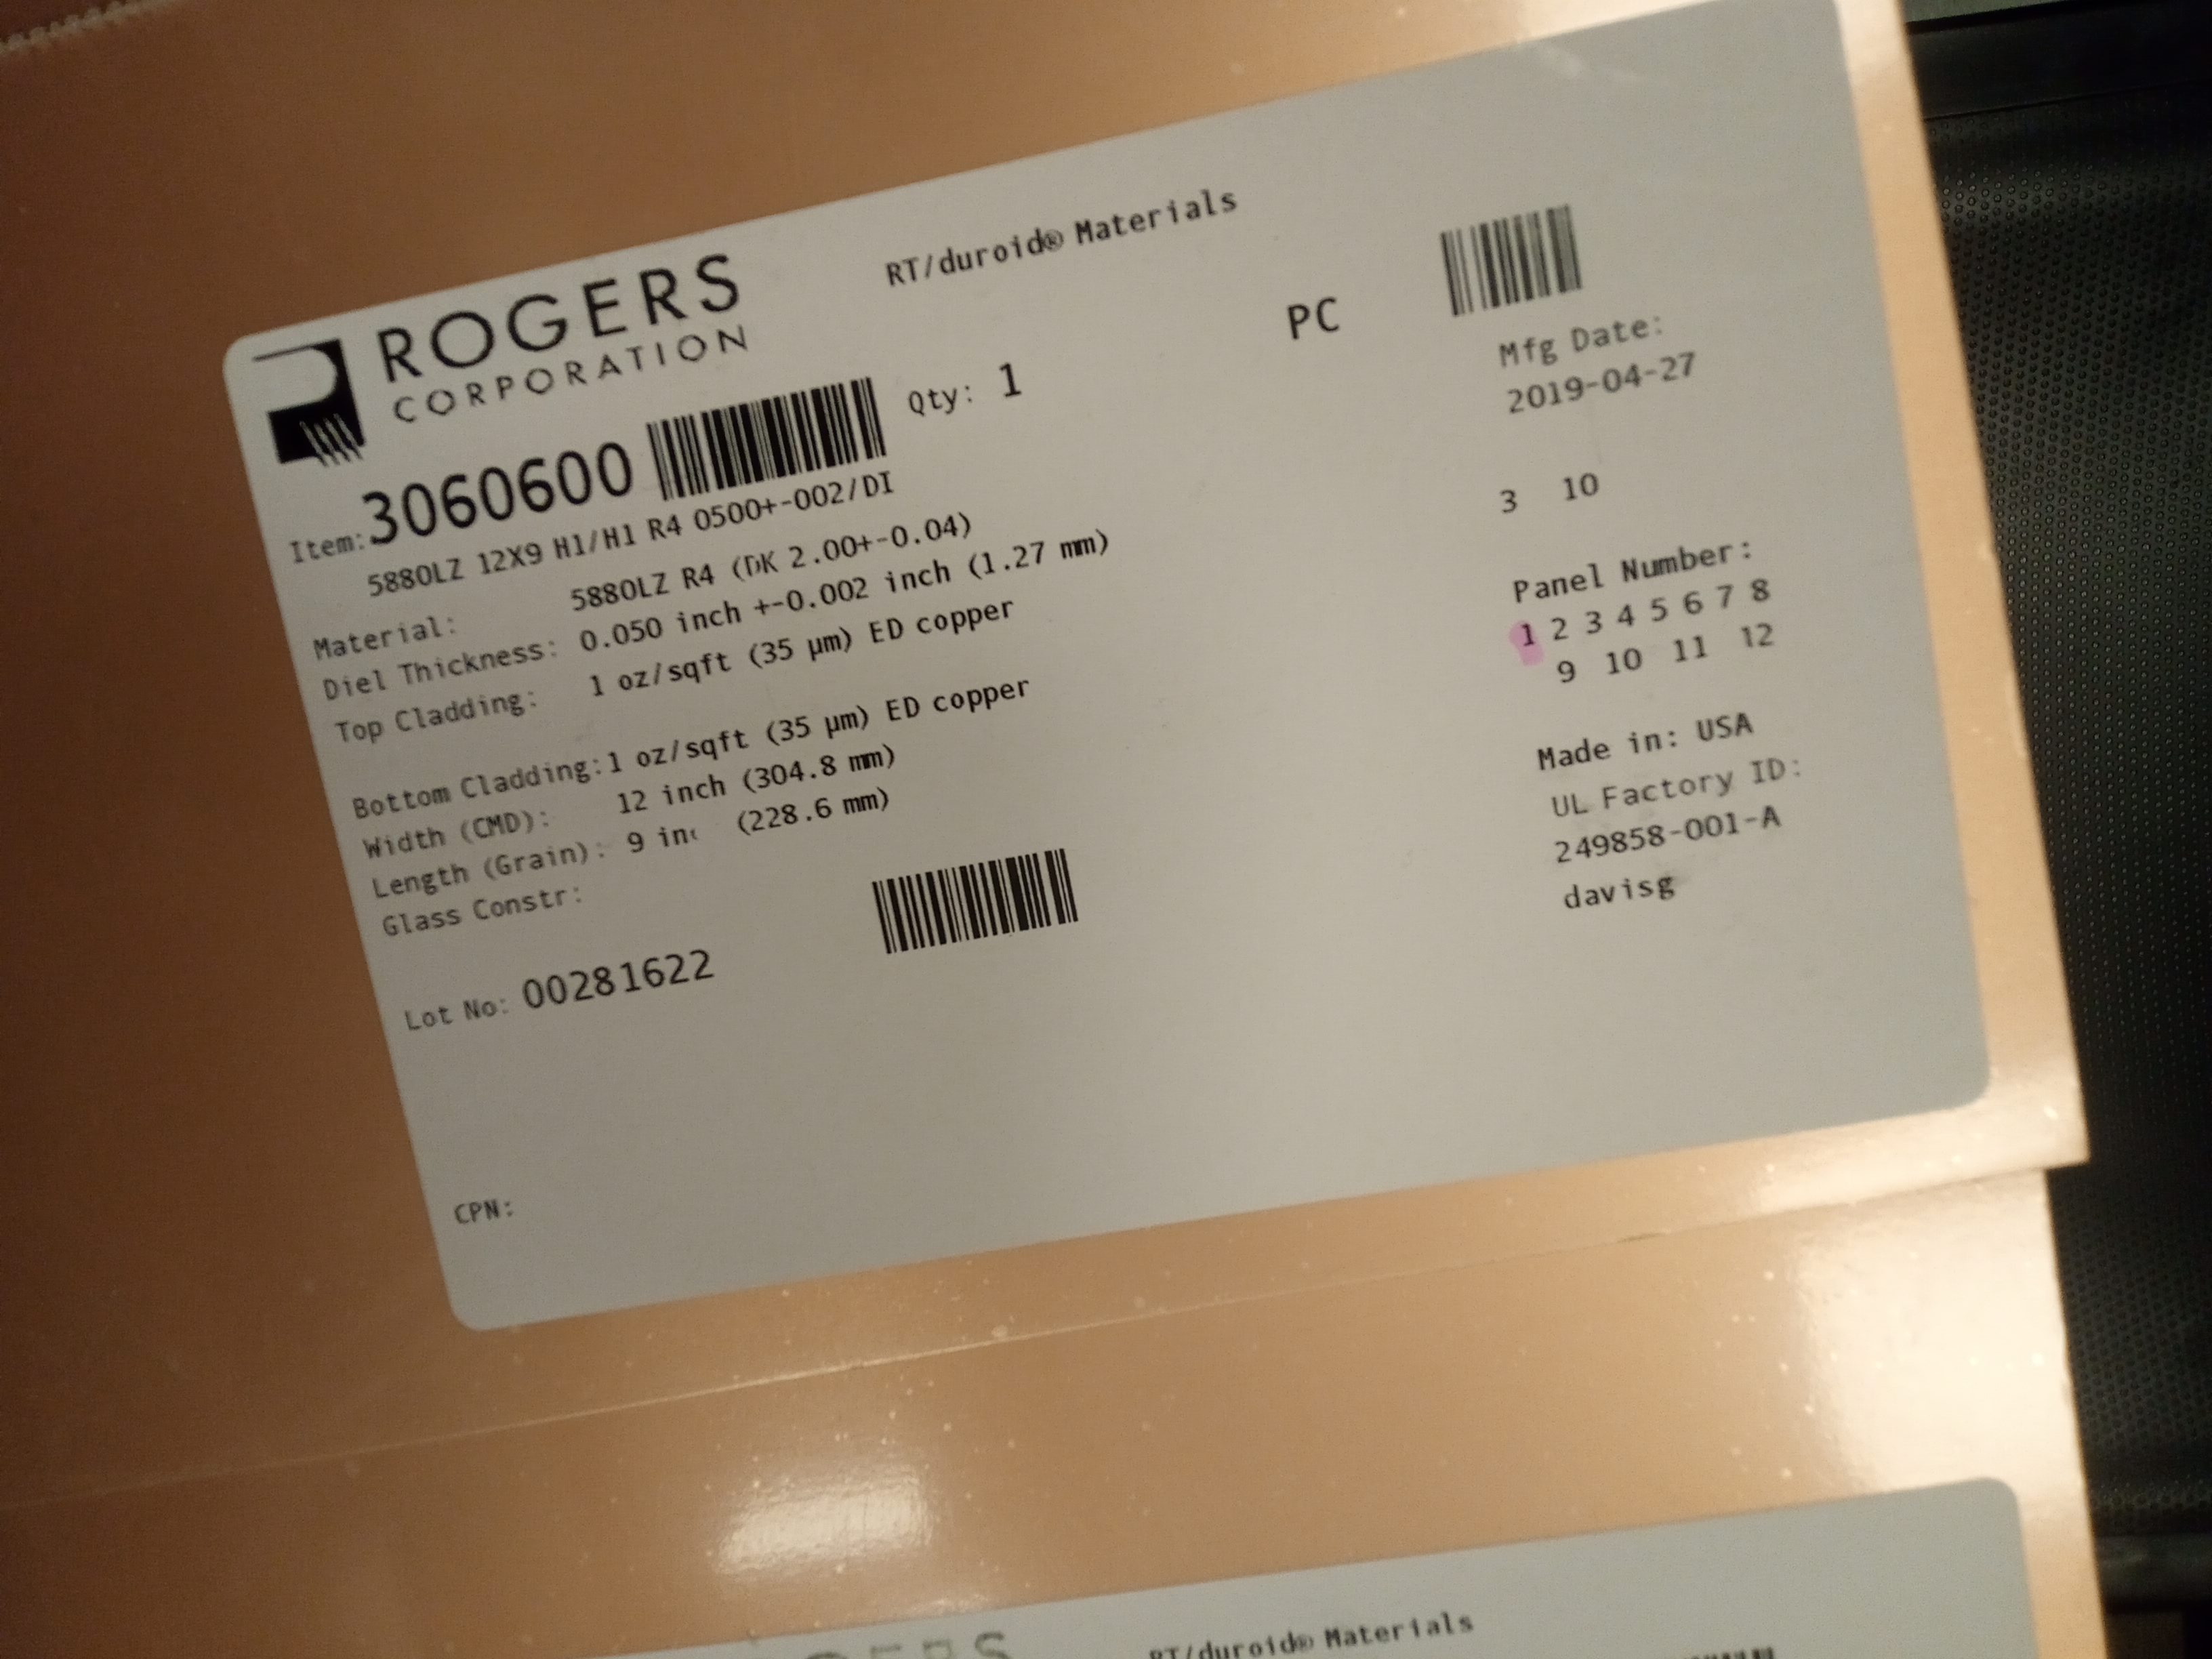
\includegraphics[width=\linewidth]{./img/sustrato.jpg}
\end{minipage}

\subsubsection*{Router CNC}
\begin{minipage}{0.32\linewidth}
    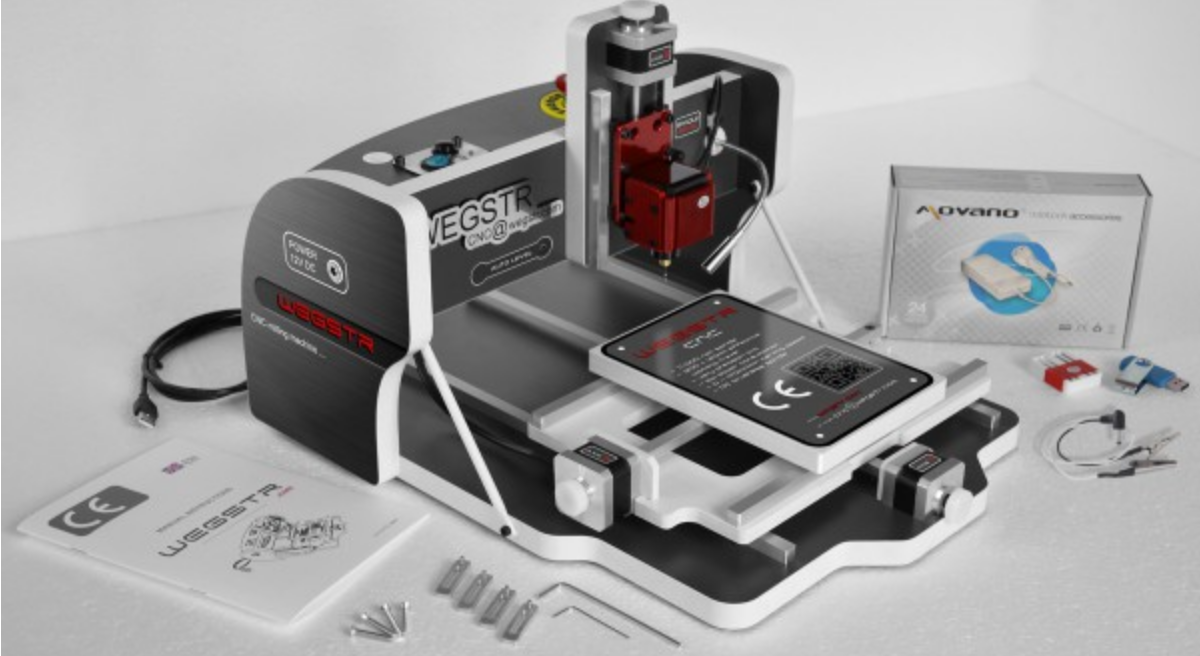
\includegraphics[width=1\linewidth]{./img/wegstr.png}
\end{minipage}
\begin{minipage}{0.66\linewidth}
La impresión sobre el PCB se hace con un router CNC marca Wegstr \cite{wegstr} con las siguientes características.
\end{minipage}
\vspace{8pt}

\begin{center}
\begin{tabular}{|l|l|}
\hline
\textbf{Parámetro} & \textbf{Valor} \\
\hline
Pasos del motor paso a paso & 0.004 mm \\
Dimensiones (X × Y × Z) & 380 × 460 × 290 mm \\
Peso & 7 kg \\
Diámetro del husillo & 3.175 mm \\
Repetitividad & 0.02 mm \\
País de origen & República Checa \\
\hline
\end{tabular}
\end{center}

\subsubsection*{Analizador de redes}

\begin{minipage}{0.4\linewidth}
  Las mediciones sobre el proyecto final con un Analizador de redes de dos puertos marca Rohde \& Schwarz modelo ZNC3-2Port \cite{RS_ZNC}
\end{minipage}
\begin{minipage}{0.59\linewidth}
  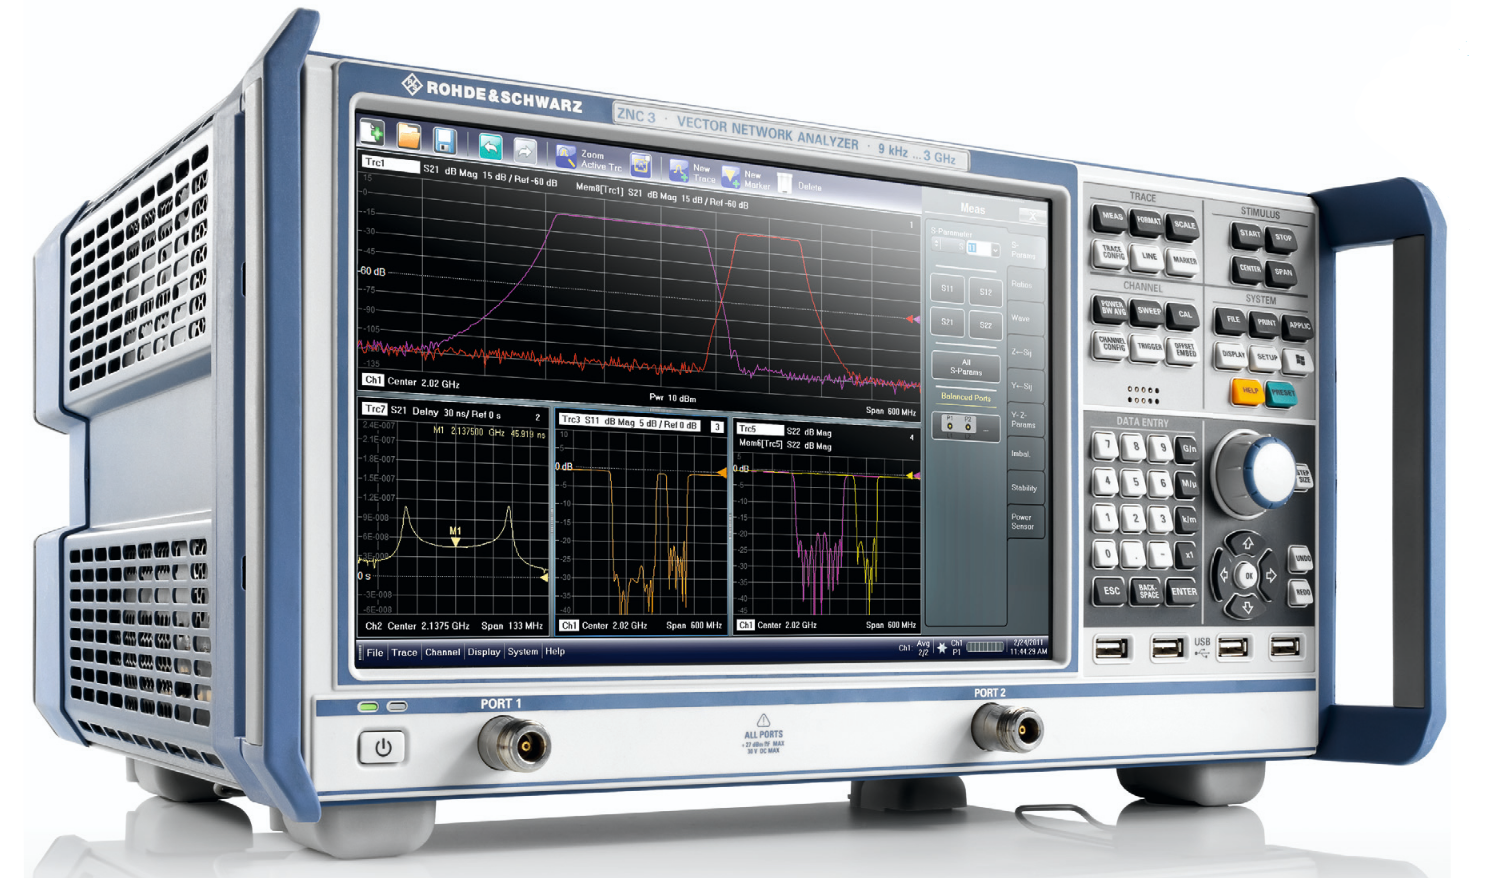
\includegraphics[width=\linewidth]{./img/vna.png}
\end{minipage}

\section*{Diseño ideal}
Primero hicimos un diagrama funcional y simulamos las relaciones entre entrada y salida.
El esquemático se diseña en ADS y se pone a continuación
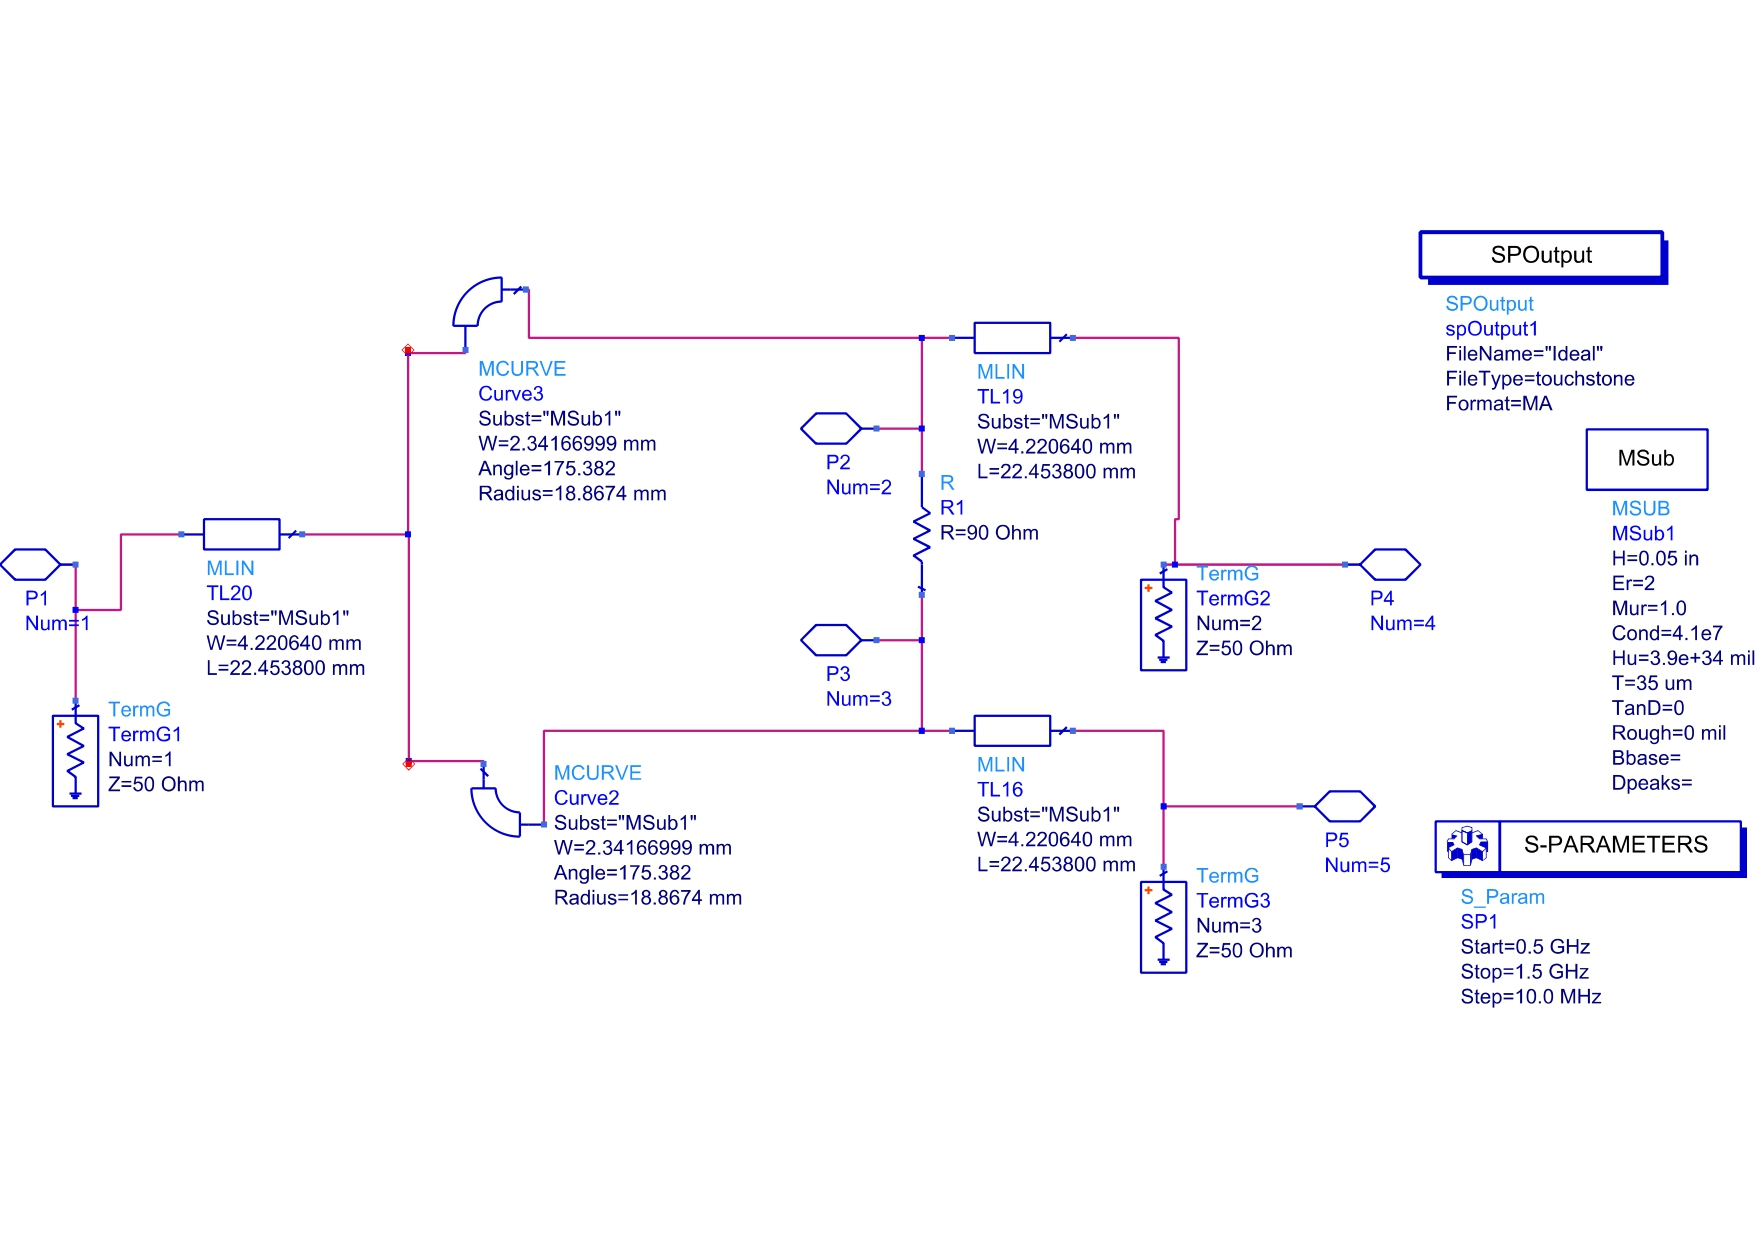
\includegraphics[width = 0.9\linewidth]{./img/ideal.jpg}

Iniciando desde el puerto uno (desde la izquierda) se tienen:

\begin{itemize}
    \item Un tramo calculado para que a $1\text{GHz}$ tenga $1\lambda$ de forma tal de ganar distancia entre el conector y la entrada a los dos transformadores de $\frac{1}{4}\lambda$ sin que haya desfasaje
    \item Dos arcos con un radio calculado de manera tal que su longitud sea $\frac{1}{4}\lambda$. Su ancho de pista se calcula con linecalc para que su impedancia sea $Z = \sqrt{2}Z_0 \approx 70.7\Omega$
    \item Dos puertos con una resistencia en el medio de $90\Omega$. Se elige este valor por limitaciones de stock en laboratorio (ideal sería $100\Omega = 2Z_0$)
    \item Luego el resto hacia la derecha son parámetros necesarios únicamente para ejecutar la simulación
\end{itemize}
Como se ve en la sección de parámetros $S$ del esquemático, la simulación se hace con un barrido de frecuencias entre $0.5$ y $1.5 \text{ GHz}$. Se simula y los resultados se exportan al formato s3p para ser procesados luego con scikit rf en Python (análisis completo al final).
Las líneas verticales gruesas en cada ploteo indican la frecuencia objetivo $1\text{GHz}$ y las líneas punteadas indican el máximo o mínimo encontrado programáticamente a partir de los datos

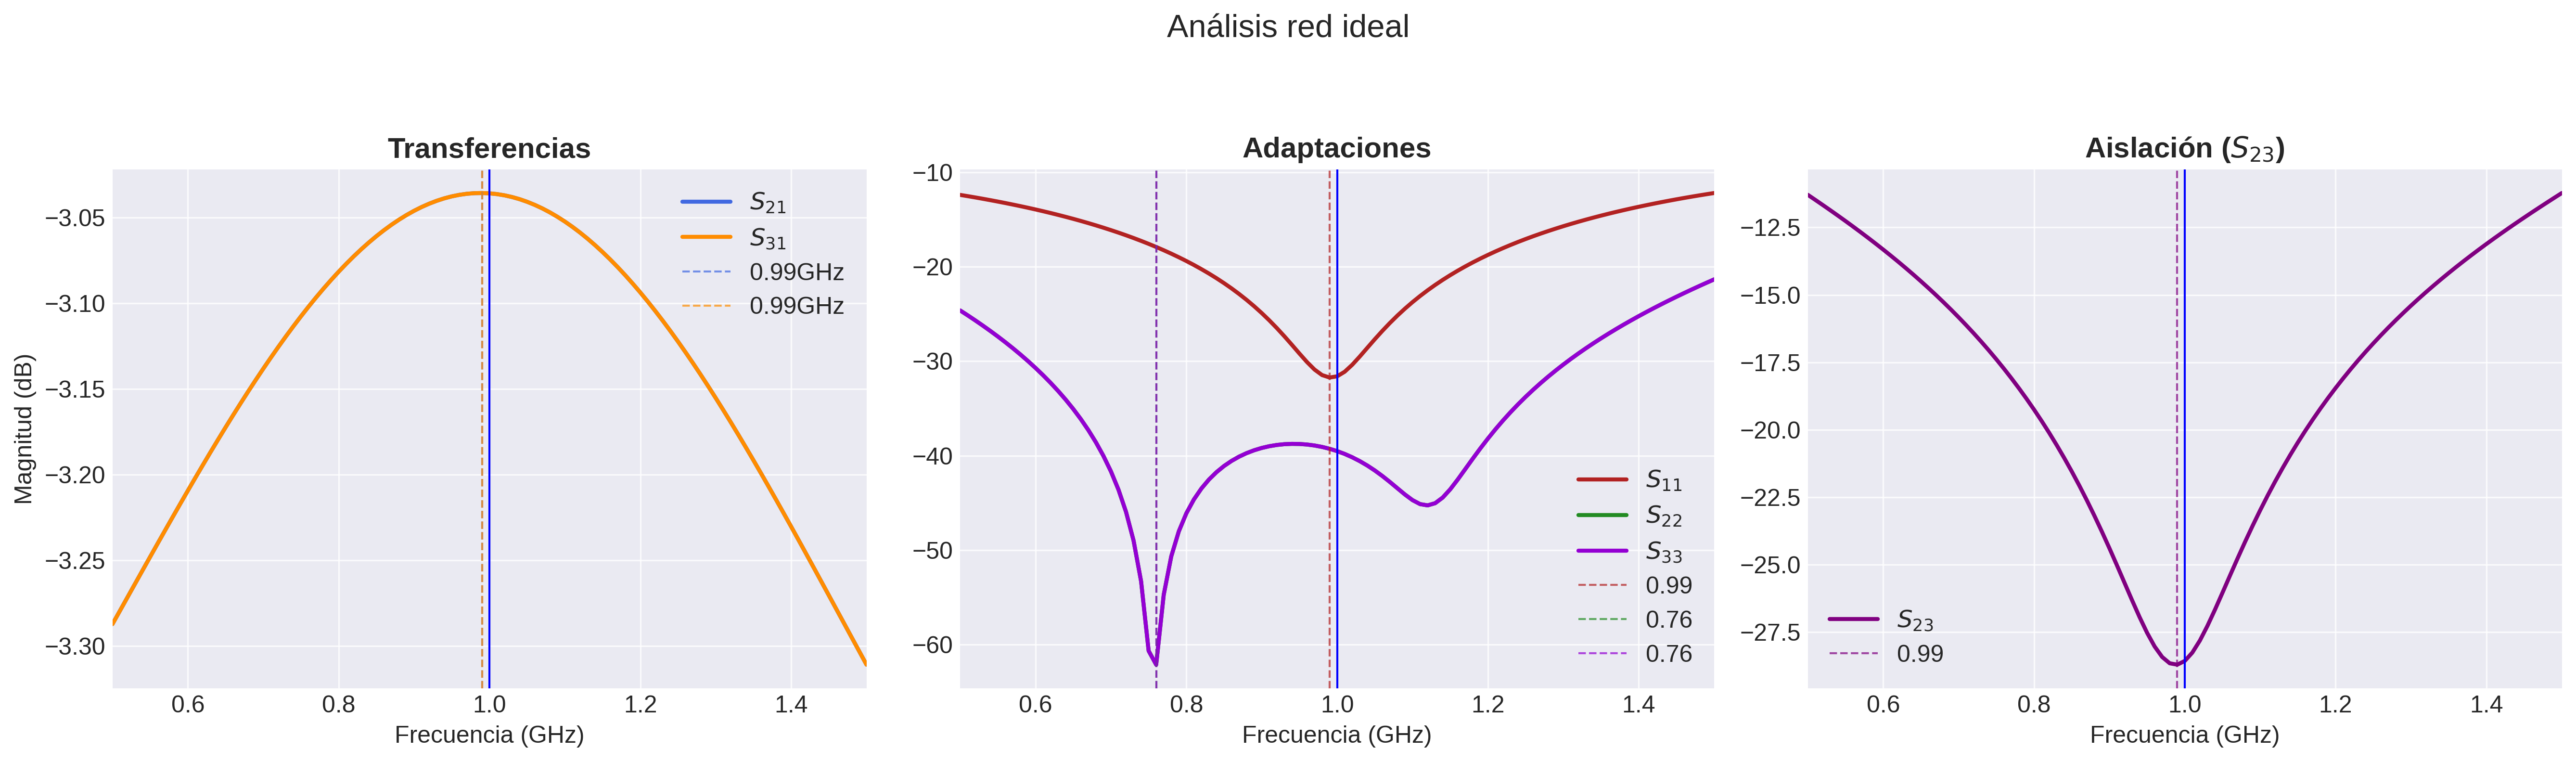
\includegraphics[width=0.9\linewidth]{./img/plot-ideal.png}

\section*{Diseño físico}
Luego se diseña el bloque físico en ADS a partir del esquemático

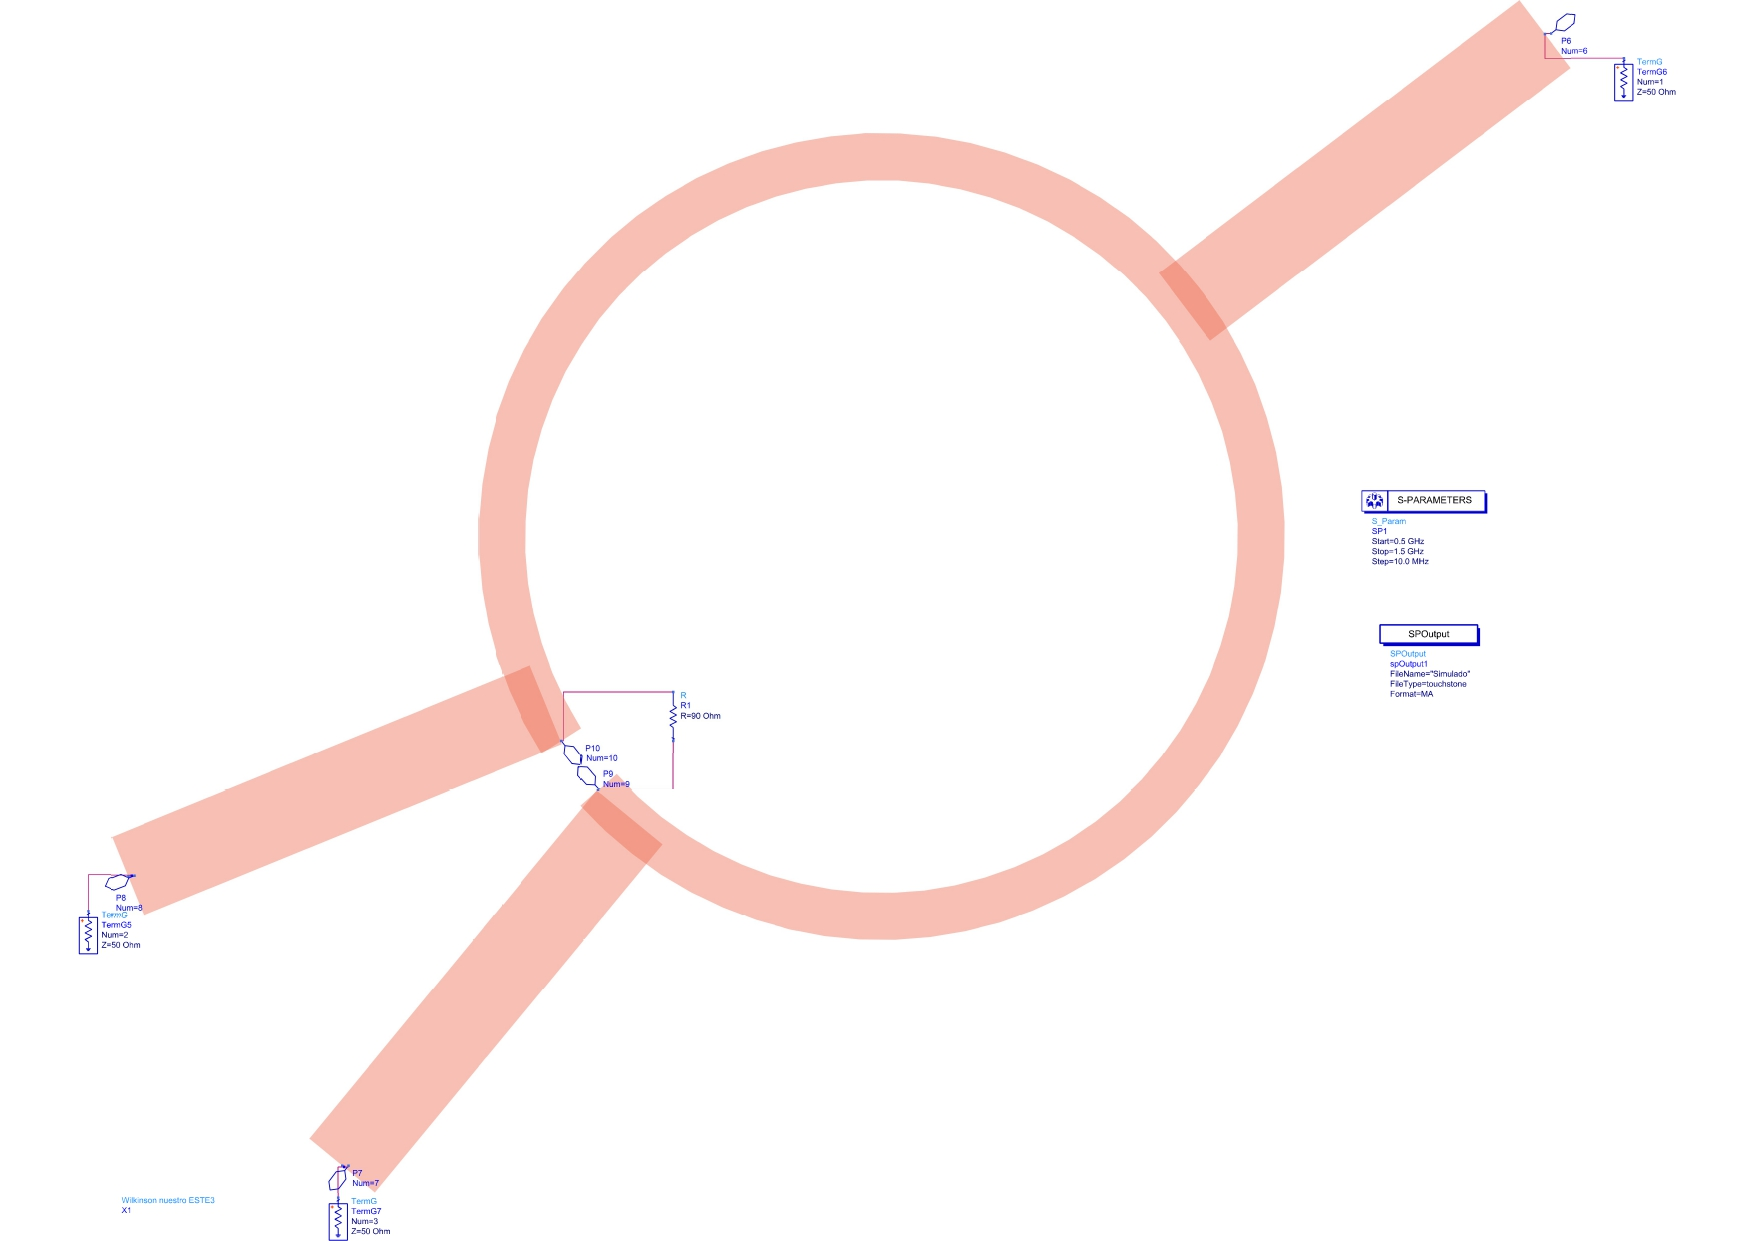
\includegraphics[width=0.6\linewidth]{./img/simulado.jpg}

La optimización de los objetivos de aislación y transferencia se logra mediante una disposición estratégica de las piezas. La selección de dos semi-círculos en lugar de tramos rectos se justifica por dos ventajas técnicas fundamentales:
\begin{itemize}
    \item Maximización de la aislación entre los tramos, reduciendo interferencias.
    \item Eliminación de ángulos agudos en el recorrido de las pistas, lo que mejora el rendimiento electromagnético del diseño.
\end{itemize}
La separación en la salida del transformador hacia los puertos viene dada por el tamaño máximo de una resistencia de radiofrecuencia que conseguimos.

Una vez definido el bloque físico, se realizan simulaciones en ADS para evaluar las transferencias. Los resultados se exportan en formato de parámetros \texttt{s3p} y se analizan mediante la metodología previamente establecida. Los datos obtenidos se presentan a continuación

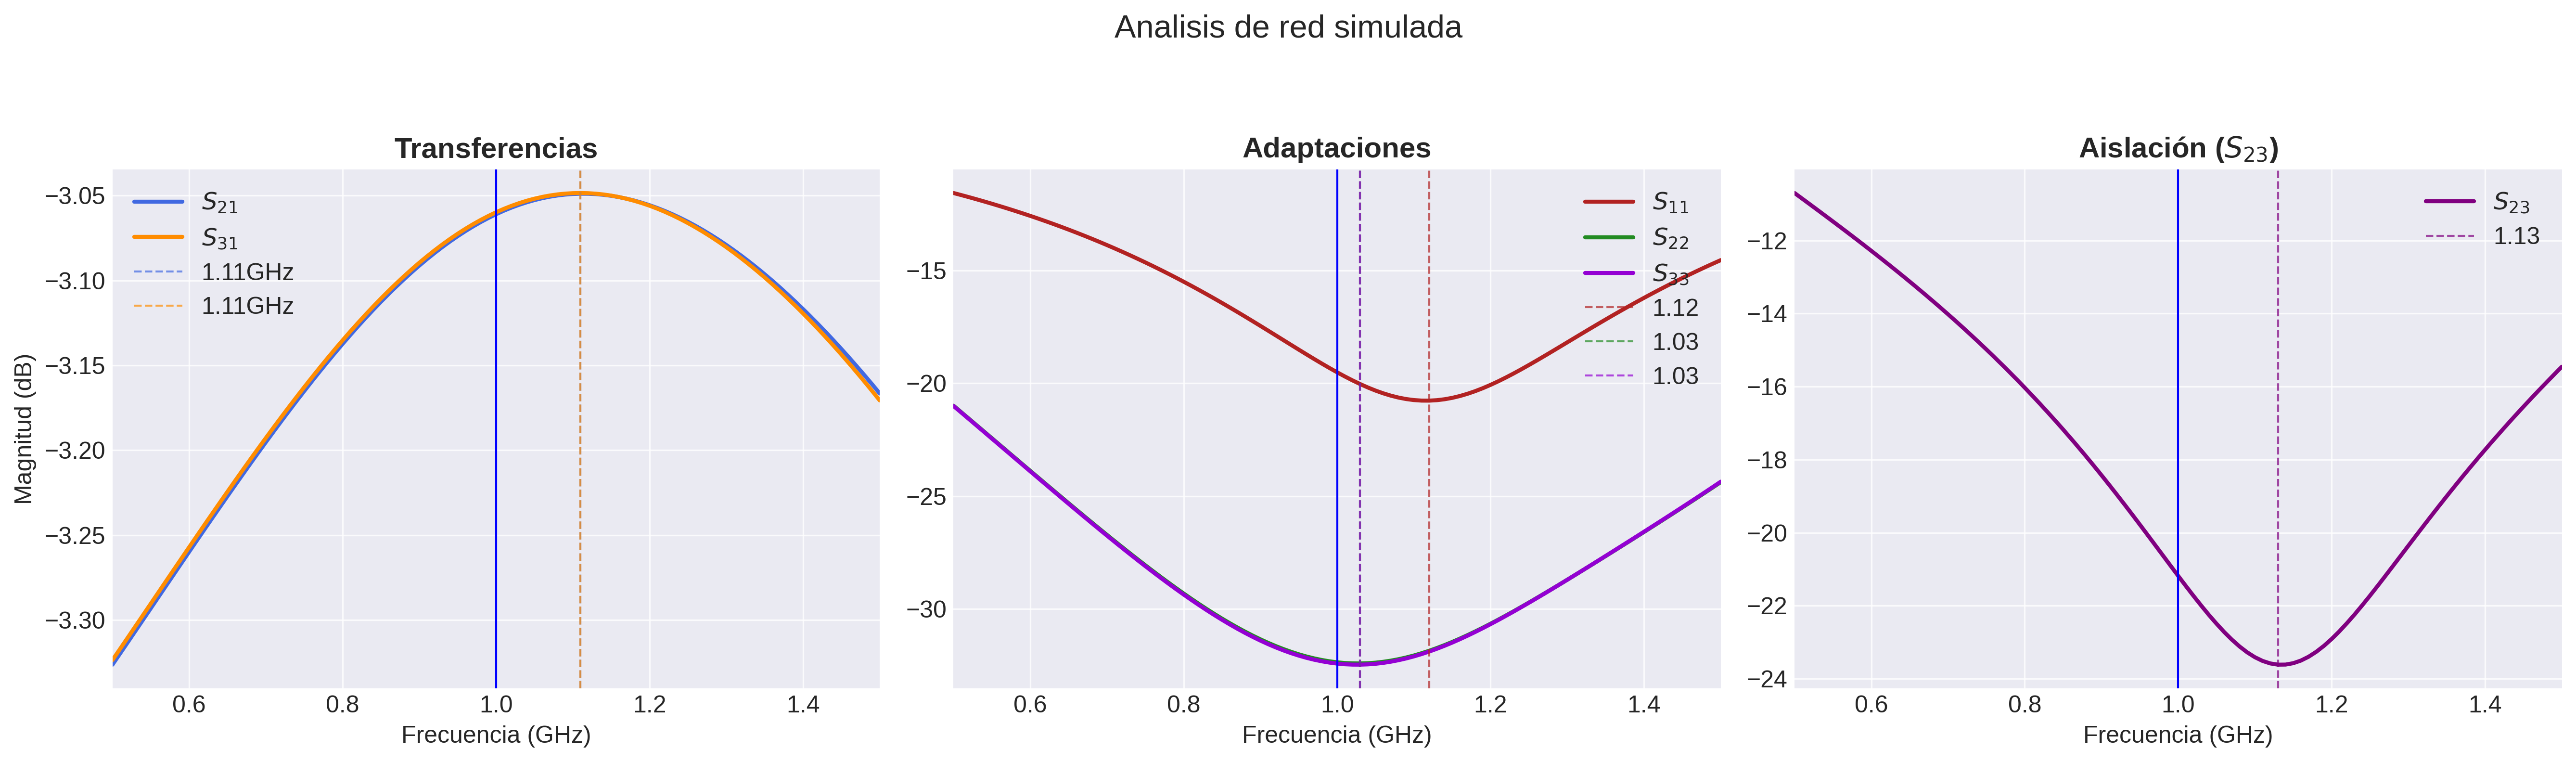
\includegraphics[width=0.9\linewidth]{./img/plot-simulado.png}

Si bien hay un claro desfasaje hacia frecuencias más altas, por limitaciónes de tiempo se determina que se mantiene el diseño.
Se detectaron dos causas posibles de error: en primera insatancia, las modificaciones manuales al diseño físico extendieron la pista del transformador de cuarto de onda. En segunda instancia, se utilizó la herramienta linecalc durante la etapa de diseño del circuito ideal, por lo que podría haberse calculado con cualquier otro substrato teórico cuyas propiedades dieléctricas permitieran mayor velocidad de desplazamiento que la correspondiente al substrato que luego utilizamos.

\section*{Construcción física}

\begin{center}
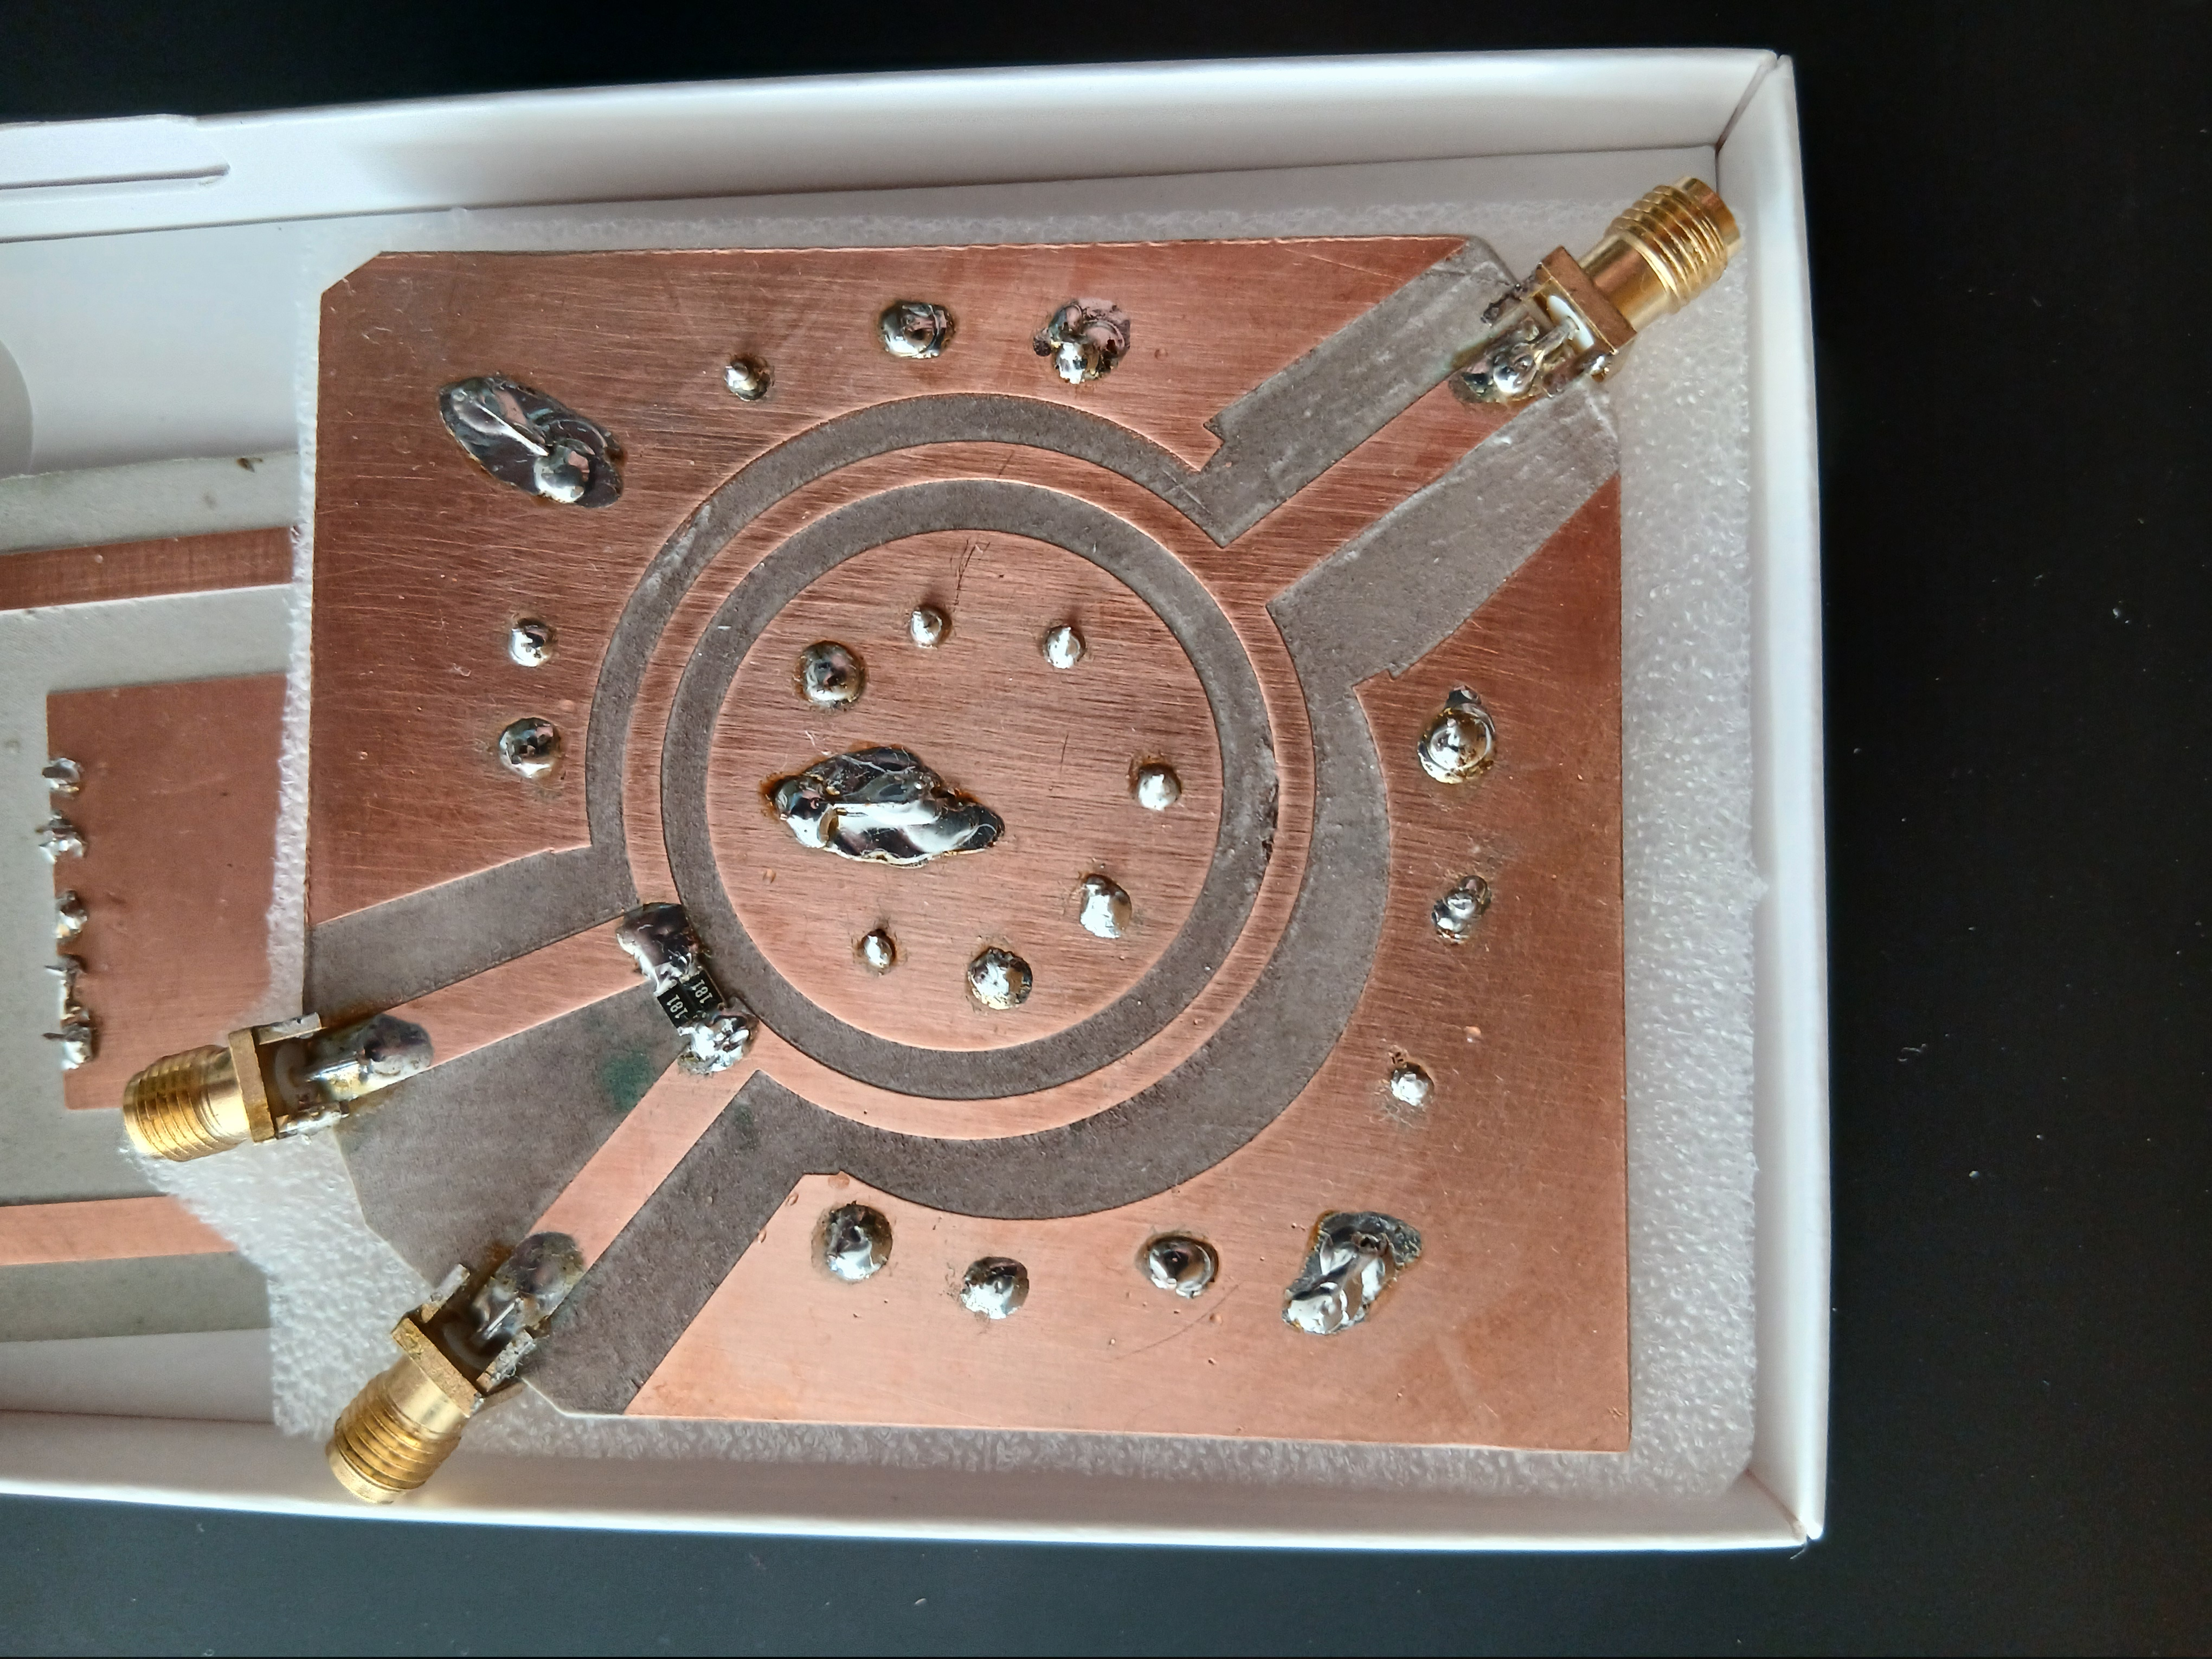
\includegraphics[width=0.7\linewidth]{./img/real.jpg}
\end{center}

\begin{minipage}{1\linewidth}
Los datos del diseño se exportan en formato Gerber para su fabricación mediante el router especificado previamente. Para reducir el desgaste de la mecha de desbaste se "dibuja" manualmente material no desbastado alrededor y en el medio del divisor con una separación entre el material de relleno (tierra) y las pistas de aproximadamente 2 anchos de pista.
Durante el ensamblado, los puertos SMA se sueldan manualmente para permitir la conexión con el analizador de redes.
Se añaden conexiónes entre el cobre que rodea a las pistas (por dentro y por fuera) y la tierra (placa de cobre inferior) evitando acoplamientos parásitos
\end{minipage}
\begin{minipage}{0.33\linewidth}

\includegraphics[width=0.99\linewidth]{./img/gerber.png}
\end{minipage}
\begin{minipage}{0.33\linewidth}
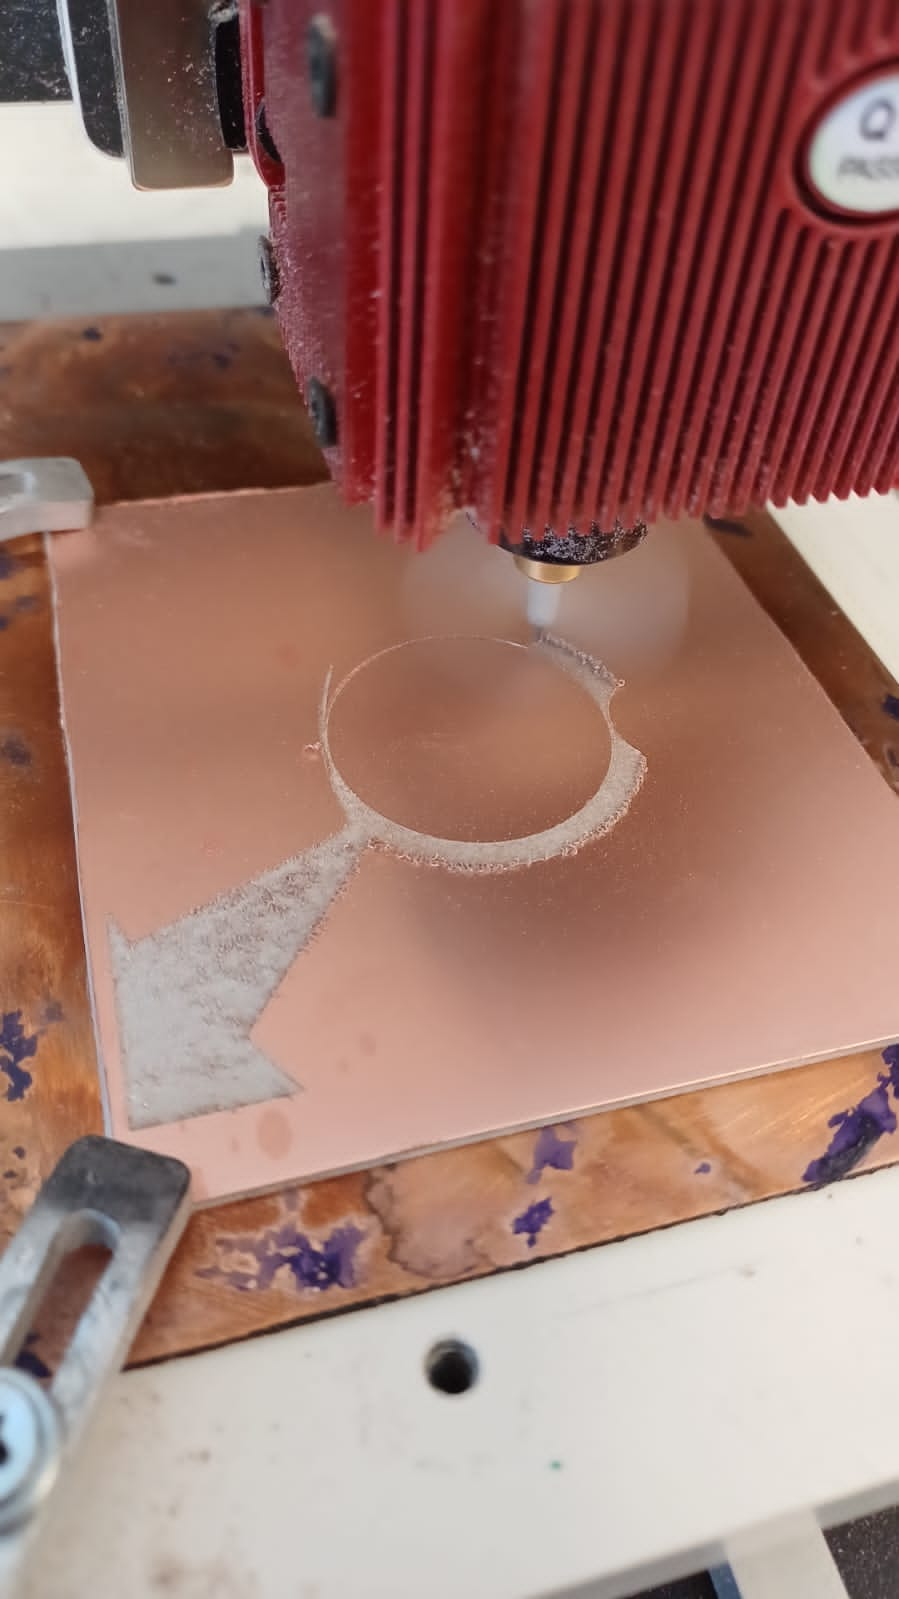
\includegraphics[width=0.99\linewidth]{./img/construccion1.jpg}
\end{minipage}
\begin{minipage}{0.33\linewidth}
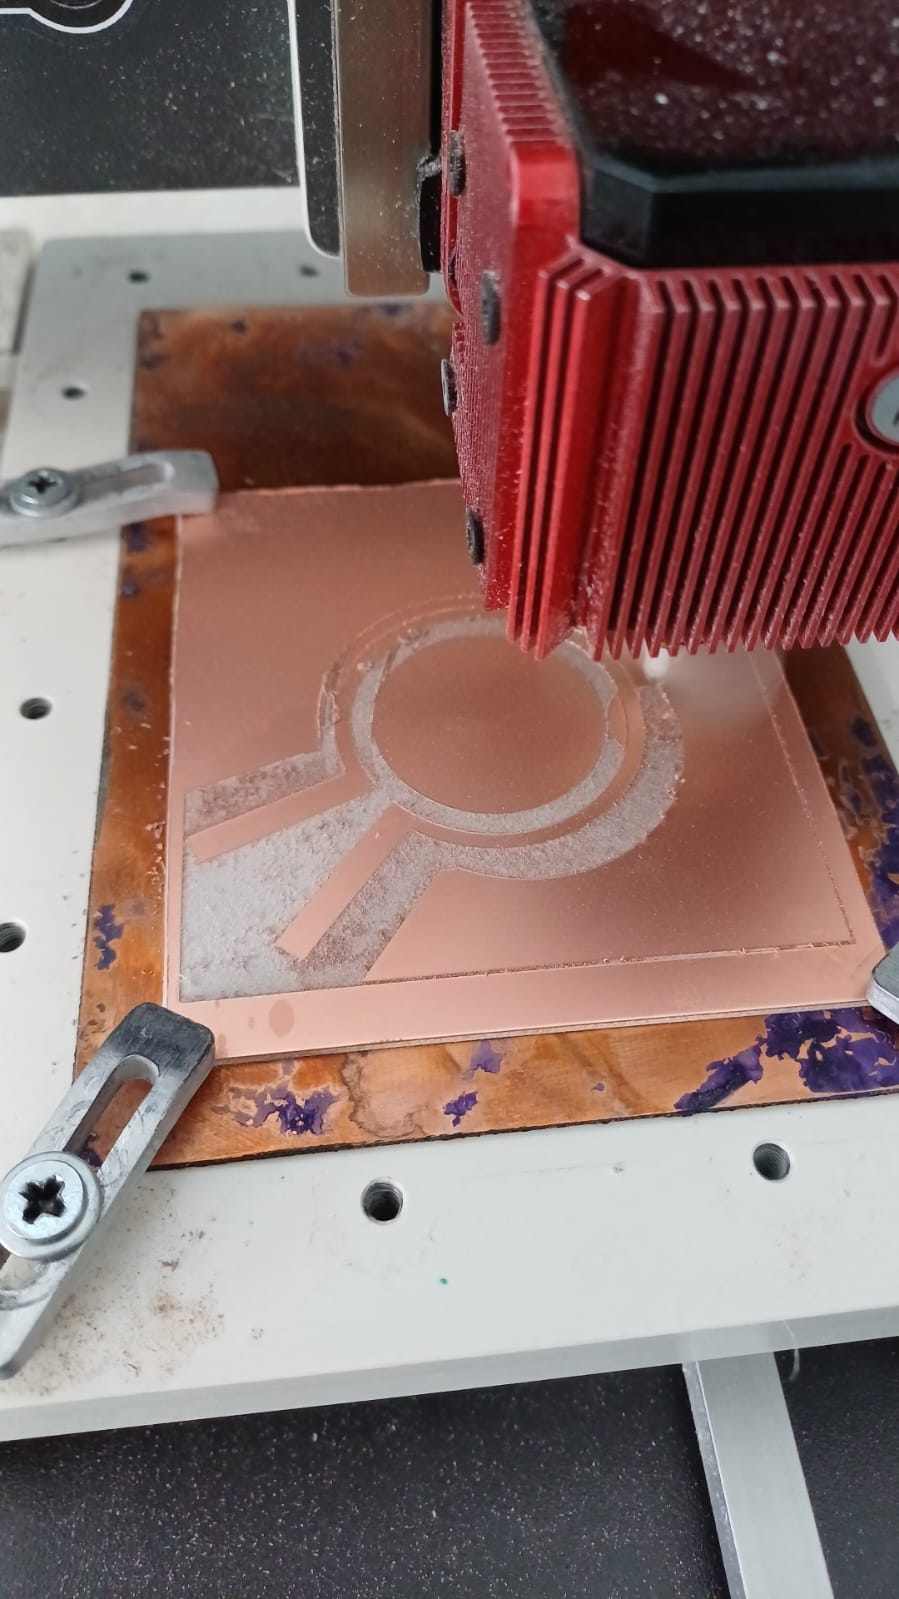
\includegraphics[width=0.99\linewidth]{./img/construccion2.jpg}
\end{minipage}

\section*{Resultados}
A continuación, se procede a realizar las mediciones utilizando el analizador de redes vectoriales (VNA) previamente especificado. Los resultados obtenidos se presentan a continuación

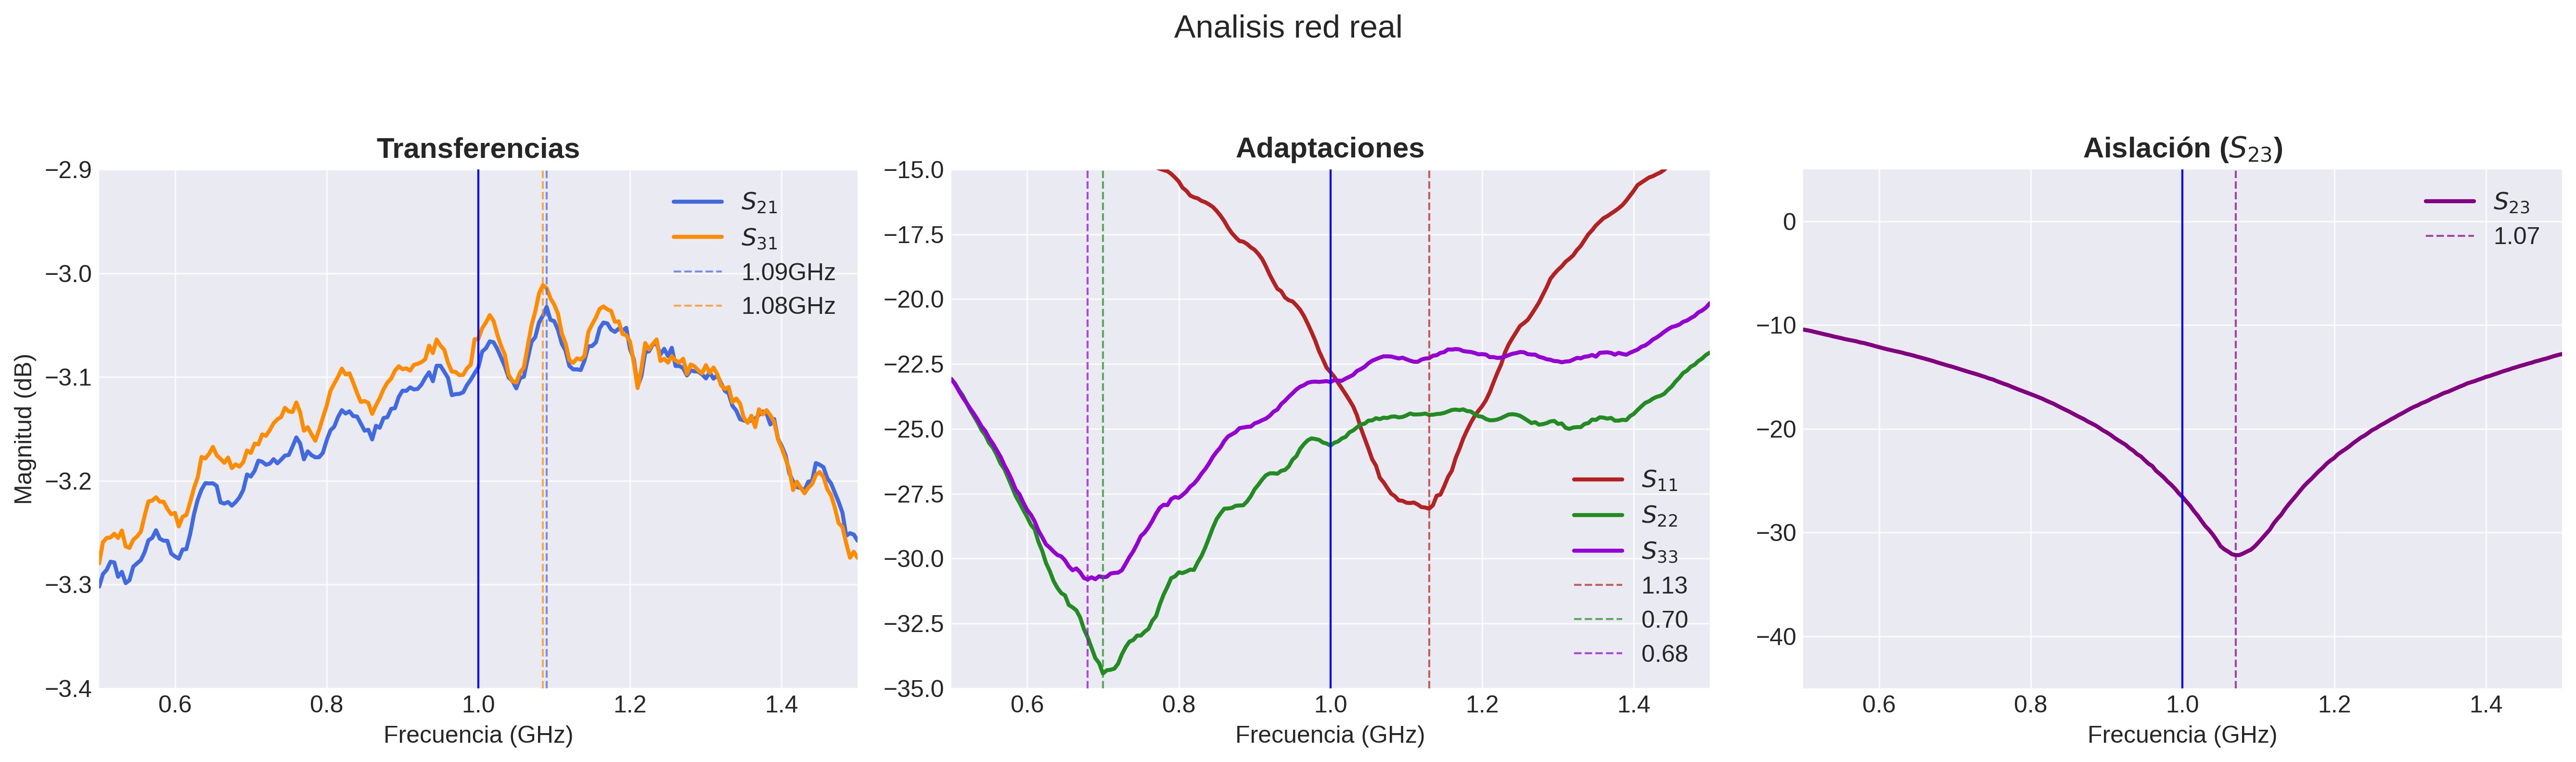
\includegraphics[width=1\linewidth]{./img/plot-real.png}

\subsection*{Resultados obtenidos vs esperados}
Los resultados muestran que el divisor cumple su función ya que en la frecuencia objetivo se tiene una relación entre entrada y salida de $\approx -3\text{dB}$ y la aislación entre los puertos de salida y las adaptaciones de los tres puertos están todas por debajo de $-20\text{dB}$. Asimismo, la toma de medición del prototipo con el VNA se correspone con los valores de la simulación del modelo físico. La construcción del prototipo resulta satisfactoria.
Se observa mucho ripple no deseado en la transferencia. Para determinar si el ripple se debía al divisor o a los cables del VNA hicimos una medición del through entre los dos cables. En el análisis anexo se hace la prueba de multiplicar los parámetros $S$ de la transferencia por la inversa del through de los cables (siempre respetando el orden de conexiones original para que los datos sean válidos) pero esto no mejora de manera sustancial el ripple si no que parece simplemente desfasarlo. Por ellos se concluye que las causas de dicho efecto se deben a errores en el aparato de medición y no al comportamiento del circuito.

A modo de autocrítica pensamos que a futuro sería bueno implementar mayor iteración en las simulaciones del bloque en el software, antes de construirlo. Si se observan las mediciones simuladas versus las reales se ve que la tendencia en el corrimiento de la máxima transferencia y máxima aislación se mantiene (se podría haber evitado).

\section*{Análisis en Scikit-rf}
Se añade como complemento el análisis hecho usando Python + Matplotlib junto con Scikit-rf en una notebook de Jupyter en el cual se analisan tanto las simulaciońes como los valores reales extraidos del VNA y se generan los ploteos puestos en este informe.

Link a repositorio en Github \url{https://github.com/SimonAulet/Analisis-Wilkinson/blob/6befe0e9da6b371b91b1758c12dfce15b5cf7c16/Analisis.ipynb}

\begin{thebibliography}{9} % El número '9' indica el ancho máximo de etiquetas (ajustar si tienes +10 ítems)
\bibitem{RS_ZNC}
Rohde \& Schwarz. \textit{ZNC Series Vector Network Analyzer Datasheet},
versión 3.02, 2022. \\
Disponible: \url{https://scdn.rohde-schwarz.com/ur/pws/dl_downloads/dl_common_library/dl_brochures_and_datasheets/pdf_1/ZNC_dat-sw_en_5214-5610-22_v0302.pdf}
\bibitem{RT-DUROID}
Sustrato. \textit{Laminados 5880LZ de RT Duroid}\\
Disponible: \url{https://www.rogerscorp.com/-/media/project/rogerscorp/documents/advanced-electronics-solutions/english/data-sheets/rt-duroid-5880lz-high-frequency-laminates.pdf}
\bibitem{wegstr}
Router para impresión
Disponible: \url{https://wegstr.com/CNC-Wegstr-LIGHT}
\end{thebibliography}

\end{document}
